\section{干预实验数字化再设计}
\subsection{既往研究}
干预实验一般考虑两个方向来确定方案。

第一个方向是实验室环境-田野环境的对抗。干预实验越接近实验室环境,其实验流程控制越严格,获取的信息越多;越接近自然环境,流程控制越松散,获取信息越少。由于实验室环境规定的流程严格,部署繁琐,成本较高,一般此类研究招募的被试人数较少,而田野实验设置在相对自然的环境当中,相对而言参与人数较多,能获得更普适的结果。

第二个方向是数字化架构-非数字化架构的对抗,数字化程度越高,所使用的数字化设备越多,反之亦然。同时,使用数字化再设计能够更方便地部署实验,并能够大幅度的减少成本方面的开支,其中涉及的研究变量被称为zero-cost variable,记为$Z$变量。
数字化实验能够几乎零成本的增加研究的人数,和实验室研究相比成本会降低很多。和现实中的田野研究相比,能够扩大调查范围,突破原先实验室设计中的时间、空间限制。

下图利用了两个坐标轴来表现这两个方向的拮抗关系。其中横坐标(x-axis)代表实验室环境-田野环境;纵坐标(y-axis)代表从低到高的数字化架构程度。

\begin{figure}[ht]
    \centering
 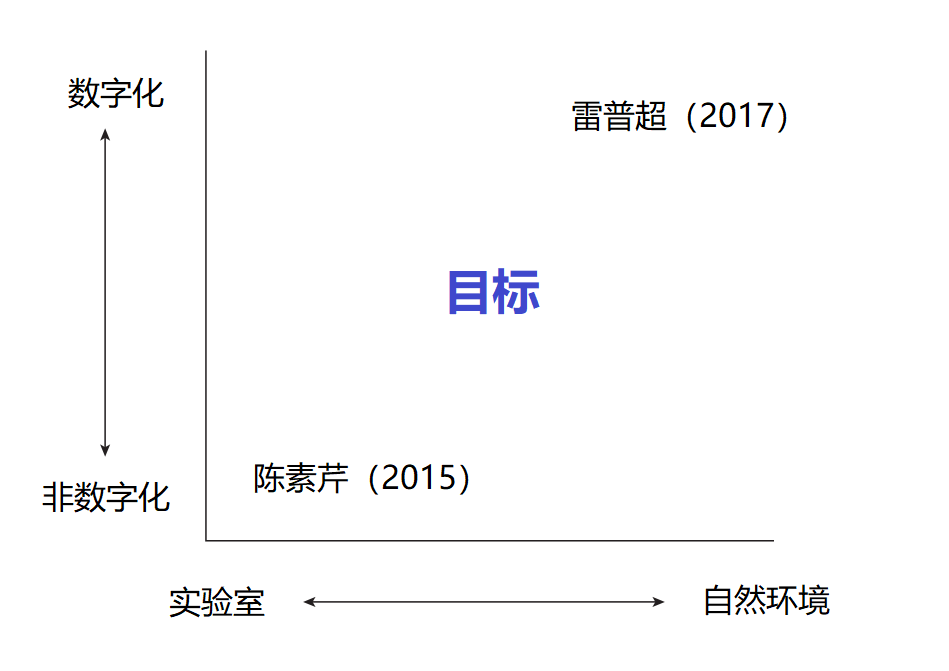
\includegraphics[scale=0.75]{digital.png}
 \caption{模式说明}
 \label{mode}
\end{figure}

我们参考了既往研究,存在大量的传统的实验室环境和田野环境知信行调研和一定数量的干预研究,而采用数字化架构的知信行干预研究知网搜索仅有14篇。我们选取了其中两个有代表性的研究作为样本对这一干预模式进行说明,分别为陈素芹2015,雷普超2018,其中陈素芹的为实验室-非数字化研究,雷普超的为田野-数字化研究。

陈素芹开展了医院COPD干预实验,实验过程完整,采用医院教育和一对一教育相结合的方式进行知信行干预,确保了病人完整经过实验流程,收集到准确的数据。但是未使用数字化架构,参与人数有限,且样本仅仅局限在某医院之内。

雷普超使用了微信公众平台进行干预实验,使用了数字化架构方便了实验的部署。但是仅仅使用了微信公众平台提供的推送功能,忽视了其他接口的使用,因此未对过程控制做出很好说明,没有能和实验参与者进行一定的反馈互动。

此外可以看出,这两个研究只进行了前测和终测(pre-post test),只是说明了知信行得分的提高,不能阐释知信行变化机制(mechanism),即是什么样的因素导致了这三者之间的相互变化。此外,陈素芹开展的实验研究成本较高,参与人数有限雷普超采用了数字化架构,但是由于对微信提供的功能利用不够,利用数字化的程度不深。此外,二者研究地点为医院、学校,受干预时间和地点限制,缺乏对于普遍人群教育的研究结果。
\subsection{混合策略创新}
如前所述,目前的知信行研究仅仅测量干预前效果和干预后的结果,并对这一结果进行直接对比,没有阐释知识、信念、行为之间变化的机制。为了探索机制(mechanisms)我们需要更多可以观测的变量,和一套可以容纳这些变量的系统。微信公众平台的一系列功能符合我们的设想。

在同样使用微信公众平台进行知信行研究的案例中,研究者仅仅使用了微信平台发消息的功能,而对于平台搜集的信息没能进行很好的利用。

微信公众平台提供图文分析、消息分析、终端分析、投票、留言等一系列功能,可以整合进实验设计当中。同时也没有利用投票功能获得期间的反馈,来对过程进行控制。这些可以为干预实验提供更多可供研究的变量。例如可以让更多时间分析相关的变量加入:地理信息、终端设备、阅读数、人数追踪等等。

我们对这样的实验设计做出一些改进,使用混合策略进行数字化再设计,既使用数字化架构,同时采取一些措施对于实验过程进行控制。在这种设计模式\ref{mode}下,我们通过微信的互动机制(投票、留言)等获知知识的习得情况和人群态度在实验过程中的累积,并试图描述在干预过程中它们是如何发生变化。

总而言之,这一混合策略牺牲了一部分实验室环境下的优点,但是提高了数字化的程度,在基于一定的过程控制策略下能够得出较为普适的结论,分述如下:
\begin{itemize}
    \item 通过标签/时间戳追踪分组
    \item 研究成本低,参与人数较多
    \item 更多利用微信提供的分析接口
    \item 打破时间和地点的限制
\end{itemize}
\subsection{实验目的和方法}
我们希望通过经过数字化再设计的知信行随机对照组实验进一步说明知识、信念、行为之间的转化关系,向治未病健康传播提供建议,并投入到已建成的平台上进行检验。

我们提出以下几个实验假设:
\begin{enumerate}
    \item 经过知信行干预后得分提高
    \item 同样强度的干预具有衰减效应,效果随时间推移减少
    \item 受监督组干预后得分较未监督组高
    \item 不同时间段阅读对干预效果无影响
\end{enumerate}

干预实验经过招募人员,随机分组,进行实验,验证假设四个步骤。
\begin{itemize}
    \item 招募:通过可靠的网络平台进行统一招募,发放一定的酬劳。
    \item 分组:随机化分组,将被试者分为监督组、未监督组、对照组三组各150人。
    \item 实验:
    
    为了验证假设1,给予各分组同时间、同频率、相同内容的推送,持续一个月。
    
        为了验证假设2,给予各分组同时间、同频率、相同内容的推送,持续三个月,每月内容和上月同期内容相同。
        
         为了验证假设3,给予各分组同时间、同频率、相同内容的推送,持续一个月,比较监督组/未监督组得分。    
         
         为了验证假设4,给予各分组不同时间、同频率、相同内容的推送,持续一个月。
        \item 验证以上假设
\end{itemize}


